\chapter{Deuteronomy 4}

\begin{figure}
  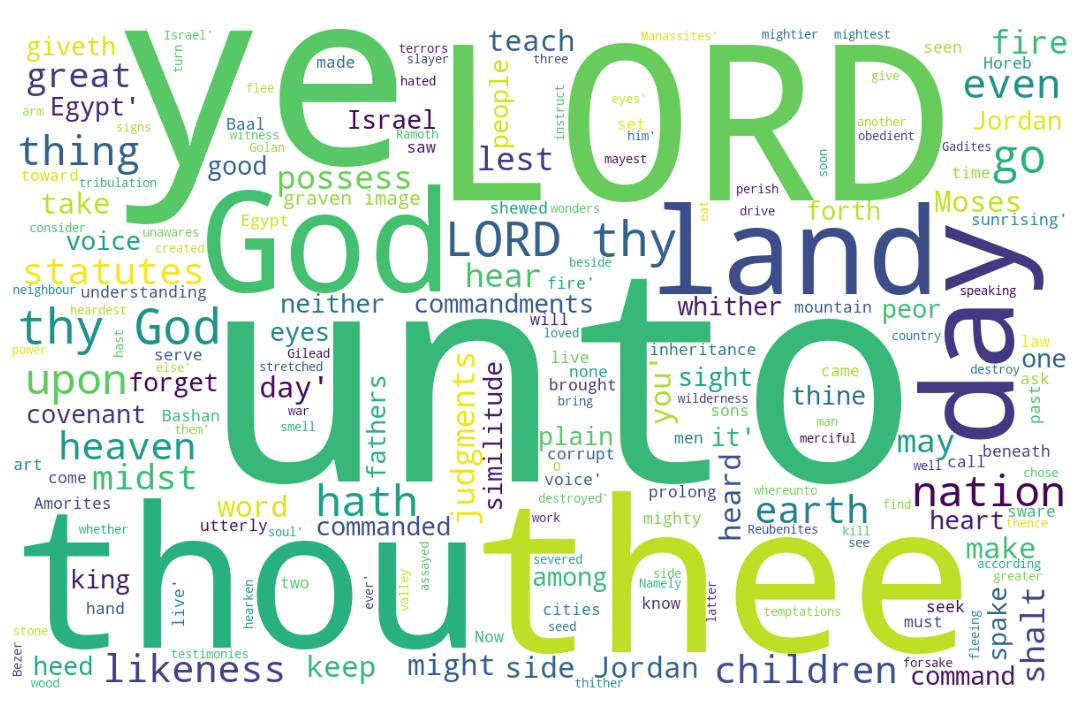
\includegraphics[width=\linewidth]{05OT-Deuteronomy/Deuteronomy4-WordCloud.jpg}
  \caption{Deuteronomy 4 Word Cloud}
  \label{fig:Deuteronomy 4 word Cloud}
\end{figure}


\marginpar{\scriptsize \centering  \fcolorbox{bone}{lime} {\textbf{BEHAVE AND BE BLESSED}}\\ (Deuteronomy 4:1-49) \begin{compactenum}[I.][8]
    \item The \textbf{Commandments} \index[scripture]{Deuteronomy!Deu 04:02}\index[scripture]{Deuteronomy!Deu 04:05}\index[scripture]{Deuteronomy!Deu 04:13}\index[scripture]{Deuteronomy!Deu 04:14}\index[scripture]{Deuteronomy!Deu 04:40} (Deu 4:2, 5, 13, 14, 40)
    \item A \textbf{Cleaving} \index[scripture]{Deuteronomy!Deu 04:04}  (Deu 4:4)
    \item The \textbf{Children} \index[scripture]{Deuteronomy!Deu 04:10}\index[scripture]{Deuteronomy!Deu 04:25}\index[scripture]{Deuteronomy!Deu 04:40}\index[scripture]{Deuteronomy!Deu 04:44}\index[scripture]{Deuteronomy!Deu 04:45}\index[scripture]{Deuteronomy!Deu 04:26} (Deu 4:10, 25, 40, 44, 45, 46)
    \item The \textbf{Covenant} \index[scripture]{Deuteronomy!Deu 04:13}\index[scripture]{Deuteronomy!Deu 04:23}\index[scripture]{Deuteronomy!Deu 04:31}  (Deu 4:13, 23, 31)
    \item The \textbf{Corruption} \index[scripture]{Deuteronomy!Deu 04:16}\index[scripture]{Deuteronomy!Deu 04:25}  (Deu 4:16, 25)
    \item A \textbf{Consideration} \index[scripture]{Deuteronomy!Dt 04:39}  (Deu 4:39)
    \item The \textbf{Cities} \index[scripture]{Deuteronomy!Deu 04:41}\index[scripture]{Deuteronomy!Deu 04:42} (Deu 4:41, 42)
\end{compactenum}}


\footnote{\textcolor[cmyk]{0.99998,1,0,0}{\hyperlink{TOC}{Return to end of Table of Contents.}}}\footnote{\href{https://audiobible.com/bible/deuteronomy_4.html}{\textcolor[cmyk]{0.99998,1,0,0}{Deuteronomy 4 Audio}}}\textcolor[cmyk]{0.99998,1,0,0}{Now therefore hearken, O Israel, unto the statutes and unto the judgments, which I teach you, for to do \emph{them}, that ye may live, and go in and possess the land which the LORD God of your fathers giveth you.}
[2] \textcolor[cmyk]{0.99998,1,0,0}{Ye shall not add unto the word which I  \fcolorbox{bone}{lime} {command} you, neither shall ye diminish \emph{ought} from it, that ye may keep the commandments of the LORD your God which I command you.}
[3] \textcolor[cmyk]{0.99998,1,0,0}{Your eyes have seen what the LORD did because of Baal-peor: for \fcolorbox{bone}{bone}{all} the men that followed Baal-peor, the LORD thy God hath destroyed them from among you.}
[4] \textcolor[cmyk]{0.99998,1,0,0}{But ye that did  \fcolorbox{bone}{lime} {cleave} unto the LORD your God \emph{are} alive every one of you this day.}
[5] \textcolor[cmyk]{0.99998,1,0,0}{Behold, I have taught you statutes and judgments, even as the LORD my God commanded me, that ye should do so in the land whither ye go to possess it.}
[6] \textcolor[cmyk]{0.99998,1,0,0}{Keep therefore and do \emph{them}; for this \emph{is} your wisdom and your \fcolorbox{bone}{MYGOLD}{understanding} in the sight of the nations, which shall hear \fcolorbox{bone}{bone}{all} these statutes, and say, Surely this great nation \emph{is} a wise and \fcolorbox{bone}{MYGOLD}{understanding} people.}
[7] \textcolor[cmyk]{0.99998,1,0,0}{For what nation \emph{is} \emph{there} \emph{so} great, who \emph{hath} God \emph{so} nigh unto them, as the LORD our God \emph{is} in \fcolorbox{bone}{bone}{all} \emph{things} \emph{that} we call upon him \emph{for}?}
[8] \textcolor[cmyk]{0.99998,1,0,0}{And what nation \emph{is} \emph{there} \emph{so} great, that hath statutes and judgments \emph{so} righteous as \fcolorbox{bone}{bone}{all} this law, which I set before you this day?}
[9] \textcolor[cmyk]{0.99998,1,0,0}{Only take heed to thyself, and keep thy soul diligently, lest thou forget the things which thine eyes have seen, and lest they depart from thy heart \fcolorbox{bone}{bone}{all} the days of thy life: but teach them thy sons, and thy sons' sons;}
[10] \textcolor[cmyk]{0.99998,1,0,0}{\emph{Specially} the day that thou stoodest before the LORD thy God in Horeb, when the LORD said unto me, Gather me the people together, and I will make them hear my words, that they may learn to fear me \fcolorbox{bone}{bone}{all} the days that they shall live upon the earth, and \emph{that} they may teach their children.}
[11] \textcolor[cmyk]{0.99998,1,0,0}{And ye came near and stood under the mountain; and the mountain burned with fire unto the midst of heaven, with darkness, clouds, and thick darkness.}
[12] \textcolor[cmyk]{0.99998,1,0,0}{And the LORD spake unto you out of the midst of the fire: ye heard the voice of the words, but saw no similitude; only \emph{ye} \emph{heard} a voice.}
[13] \textcolor[cmyk]{0.99998,1,0,0}{And he declared unto you his  \fcolorbox{bone}{lime} {covenant}, which he  \fcolorbox{bone}{lime} {commanded} you to perform, \emph{even} ten  \fcolorbox{bone}{lime} {commandments}; and he wrote them upon two tables of stone.}\\
\\
\P \textcolor[cmyk]{0.99998,1,0,0}{And the LORD  \fcolorbox{bone}{lime} {commanded} me at that time to teach you statutes and judgments, that ye might do them in the land whither ye go over to possess it.}
[15] \textcolor[cmyk]{0.99998,1,0,0}{Take ye therefore good heed unto yourselves; for ye saw no manner of similitude on the day \emph{that} the LORD spake unto you in Horeb out of the midst of the fire:}
[16] \textcolor[cmyk]{0.99998,1,0,0}{Lest ye  \fcolorbox{bone}{lime} {corrupt} \emph{yourselves}, and make you a graven image, the similitude of any figure, the likeness of male or female,}
[17] \textcolor[cmyk]{0.99998,1,0,0}{The likeness of any beast that \emph{is} on the earth, the likeness of any winged fowl that flieth in the air,}
[18] \textcolor[cmyk]{0.99998,1,0,0}{The likeness of any thing that creepeth on the ground, the likeness of any fish that \emph{is} in the waters beneath the earth:}
[19] \textcolor[cmyk]{0.99998,1,0,0}{And lest thou lift up thine eyes unto heaven, and when thou seest the sun, and the moon, and the stars, \emph{even} \fcolorbox{bone}{bone}{all} the host of heaven, shouldest be driven to worship them, and serve them, which the LORD thy God hath divided unto \fcolorbox{bone}{bone}{all} nations under the whole heaven.}
[20] \textcolor[cmyk]{0.99998,1,0,0}{But the LORD hath taken you, and brought you forth out of the iron furnace, \emph{even} out of Egypt, to be unto him a people of inheritance, as \emph{ye} \emph{are} this day.}
[21] \textcolor[cmyk]{0.99998,1,0,0}{Furthermore the LORD was angry with me for your sakes, and sware that I should not go over Jordan, and that I should not go in unto that good land, which the LORD thy God giveth thee \emph{for} an inheritance:}
[22] \textcolor[cmyk]{0.99998,1,0,0}{But I must die in this land, I must not go over Jordan: but ye shall go over, and possess that good land.}
[23] \textcolor[cmyk]{0.99998,1,0,0}{Take heed unto yourselves, lest ye forget the  \fcolorbox{bone}{lime} {covenant} of the LORD your God, which he made with you, and make you a graven image, \emph{or} the likeness of any \emph{thing}, which the LORD thy God hath forbidden thee.}
[24] \textcolor[cmyk]{0.99998,1,0,0}{For the LORD thy God \emph{is} a consuming fire, \emph{even} a jealous God.}\footnote{\textbf{Deuteronomy 9:3} - Understand therefore this day, that the LORD thy God is he which goeth over before thee; as a consuming fire he shall destroy them, and he shall bring them down before thy face: so shalt thou drive them out, and destroy them quickly, as the LORD hath said unto thee.}\footnote{\textbf{Hebrews 12:29} - For our God is a consuming fire.}\\
\\
\P \textcolor[cmyk]{0.99998,1,0,0}{When thou shalt beget children, and children's children, and ye shall have remained long in the land, and shall  \fcolorbox{bone}{lime} {corrupt} \emph{yourselves}, and make a graven image, \emph{or} the likeness of any \emph{thing}, and shall do evil in the sight of the LORD thy God, to provoke him to anger:}
[26] \textcolor[cmyk]{0.99998,1,0,0}{I call heaven and earth to witness against you this day, that ye shall soon utterly perish from off the land whereunto ye go over Jordan to possess it; ye shall not prolong \emph{your} days upon it, but shall utterly be destroyed.}
[27] \textcolor[cmyk]{0.99998,1,0,0}{And the LORD shall scatter you among the nations, and ye shall be left few in number among the heathen, whither the LORD shall lead you.}
[28] \textcolor[cmyk]{0.99998,1,0,0}{And there ye shall serve gods, the work of men's hands, wood and stone, which neither see, nor hear, nor eat, nor smell.}
[29] \textcolor[cmyk]{0.99998,1,0,0}{But if from thence thou shalt seek the LORD thy God, thou shalt find \emph{him}, if thou seek him with \fcolorbox{bone}{bone}{all} thy heart and with \fcolorbox{bone}{bone}{all} thy soul.}
[30] \textcolor[cmyk]{0.99998,1,0,0}{When thou art in tribulation, and \fcolorbox{bone}{bone}{all} these things are come upon thee, \emph{even} in the latter days, if thou turn to the LORD thy God, and shalt be obedient unto his voice;}
[31] \textcolor[cmyk]{0.99998,1,0,0}{(For the LORD thy God \emph{is} a merciful God;) he will not forsake thee, neither destroy thee, nor forget the  \fcolorbox{bone}{lime} {covenant} of thy fathers which he sware unto them.}
[32] \textcolor[cmyk]{0.99998,1,0,0}{For ask now of the days that are past, which were before thee, since the day that God created man upon the earth, and \emph{ask} from the one side of heaven unto the other, whether there hath been \emph{any} \emph{such} \emph{thing} as this great thing \emph{is}, or hath been heard like it?}
[33] \textcolor[cmyk]{0.99998,1,0,0}{Did \emph{ever} people hear the voice of God speaking out of the midst of the fire, as thou hast heard, and live?}
[34] \textcolor[cmyk]{0.99998,1,0,0}{Or hath God assayed to go \emph{and} take him a nation from the midst of \emph{another} nation, by temptations, by signs, and by wonders, and by war, and by a mighty hand, and by a stretched out arm, and by great terrors, according to \fcolorbox{bone}{bone}{all} that the LORD your God did for you in Egypt before your eyes?}
[35] \textcolor[cmyk]{0.99998,1,0,0}{Unto thee it was shewed, that thou mightest know that the LORD he \emph{is} God; \emph{there} \emph{is} none else beside him.}
[36] \textcolor[cmyk]{0.99998,1,0,0}{Out of heaven he made thee to hear his voice, that he might instruct thee: and upon earth he shewed thee his great fire; and thou heardest his words out of the midst of the fire.}
[37] \textcolor[cmyk]{0.99998,1,0,0}{And because he loved thy fathers, therefore he chose their seed after them, and brought thee out in his sight with his mighty power out of Egypt;}
[38] \textcolor[cmyk]{0.99998,1,0,0}{To drive out nations from before thee greater and mightier than thou \emph{art}, to bring thee in, to give thee their land \emph{for} an inheritance, as \emph{it} \emph{is} this day.}
[39] \textcolor[cmyk]{0.99998,1,0,0}{Know therefore this day, and  \fcolorbox{bone}{lime} {consider} \emph{it} in thine heart, that the LORD he \emph{is} God in heaven above, and upon the earth beneath: \emph{there} \emph{is} none else.}
[40] \textcolor[cmyk]{0.99998,1,0,0}{Thou shalt keep therefore his statutes, and his  \fcolorbox{bone}{lime} {commandments}, which I  \fcolorbox{bone}{lime} {command} thee this day, that it may go well with thee, and with thy children after thee, and that thou mayest prolong \emph{thy} days upon the earth, which the LORD thy God giveth thee, for ever.}\\
\\
\P \textcolor[cmyk]{0.99998,1,0,0}{Then Moses severed three  \fcolorbox{bone}{lime} {cities} on this side Jordan toward the sunrising;}
[42] \textcolor[cmyk]{0.99998,1,0,0}{That the slayer might flee thither, which should kill his neighbour unawares, and hated him not in times past; and that fleeing unto one of these  \fcolorbox{bone}{lime} {cities} he might live:}
[43] \textcolor[cmyk]{0.99998,1,0,0}{\emph{Namely}, Bezer in the wilderness, in the plain country, of the Reubenites; and Ramoth in Gilead, of the Gadites; and Golan in Bashan, of the Manassites.}\\
\\
\P \textcolor[cmyk]{0.99998,1,0,0}{And this \emph{is} the law which Moses set before the children of Israel:}
[45] \textcolor[cmyk]{0.99998,1,0,0}{These \emph{are} the testimonies, and the statutes, and the judgments, which Moses spake unto the children of Israel, after they came forth out of Egypt,}
[46] \textcolor[cmyk]{0.99998,1,0,0}{On this side Jordan, in the valley over against Beth-peor, in the land of Sihon king of the Amorites, who dwelt at Heshbon, whom Moses and the children of Israel smote, after they were come forth out of Egypt:}
[47] \textcolor[cmyk]{0.99998,1,0,0}{And they possessed his land, and the land of Og king of Bashan, two kings of the Amorites, which \emph{were} on this side Jordan toward the sunrising;}
[48] \textcolor[cmyk]{0.99998,1,0,0}{From Aroer, which \emph{is} by the bank of the river Arnon, even unto mount Sion, which \emph{is} Hermon,}
[49] \textcolor[cmyk]{0.99998,1,0,0}{And \fcolorbox{bone}{bone}{all} the plain on this side Jordan eastward, even unto the sea of the plain, under the springs of Pisgah.}